\chapter{Case Study}

This chapter introduces the XV Application (XVA) as the research case study in order to illustrate the application of multi-tenancy to a real world SaaS application as example. It aims to define a concrete set of design inputs and requirements combined with the current context of the XV SaaS application and attempts to use it as premise for architecting our multi-tenant model.

\begin{figure}
\centering
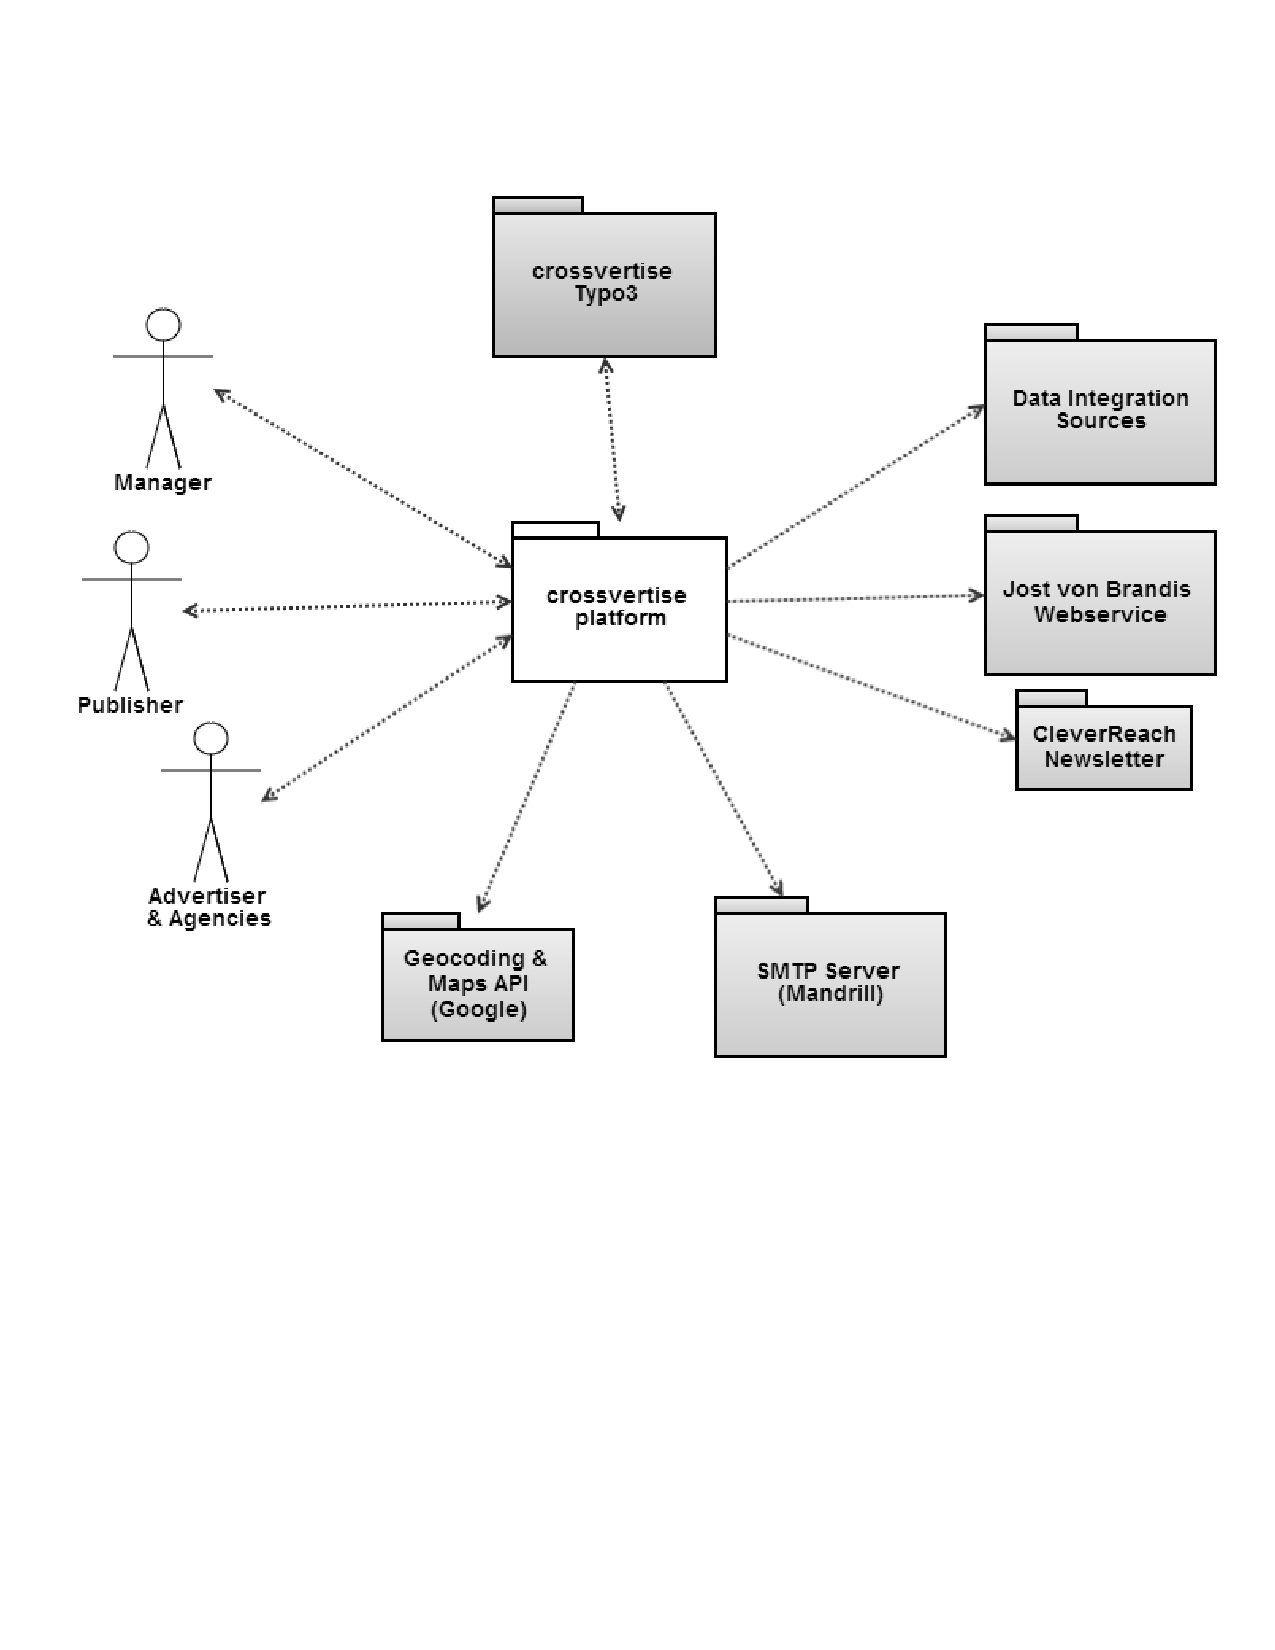
\includegraphics[width=\textwidth]{cross_use_case}
\caption{XV Use Case!!!!!!!!!!!!!!!!!!!!!!!!!!}
\label{fig:cross_use_case}
\end{figure}

\section{XV GmbH}

Crossvertise GmbH henceforth "XV", is a Munich based SaaS provider and start-up. Their core domain of business consists of the entirety of the advertising market. The company has developed their own online, cross-media marketplace application which is offered as SaaS solution to large advertising houses and corporations. Their application is also the back end of their own market.XV.com website which allows publishers, advertisers and companies to run cross-media marketing campaigns by booking advertising media online.
 
The XV Application (XVA) integrates over 80\% of Germany's advertising and publishing data to enable its users to book mobile, online, cinema, television, radio or out-of-home advertising easily and effortlessly online.

\begin{figure}
\centering
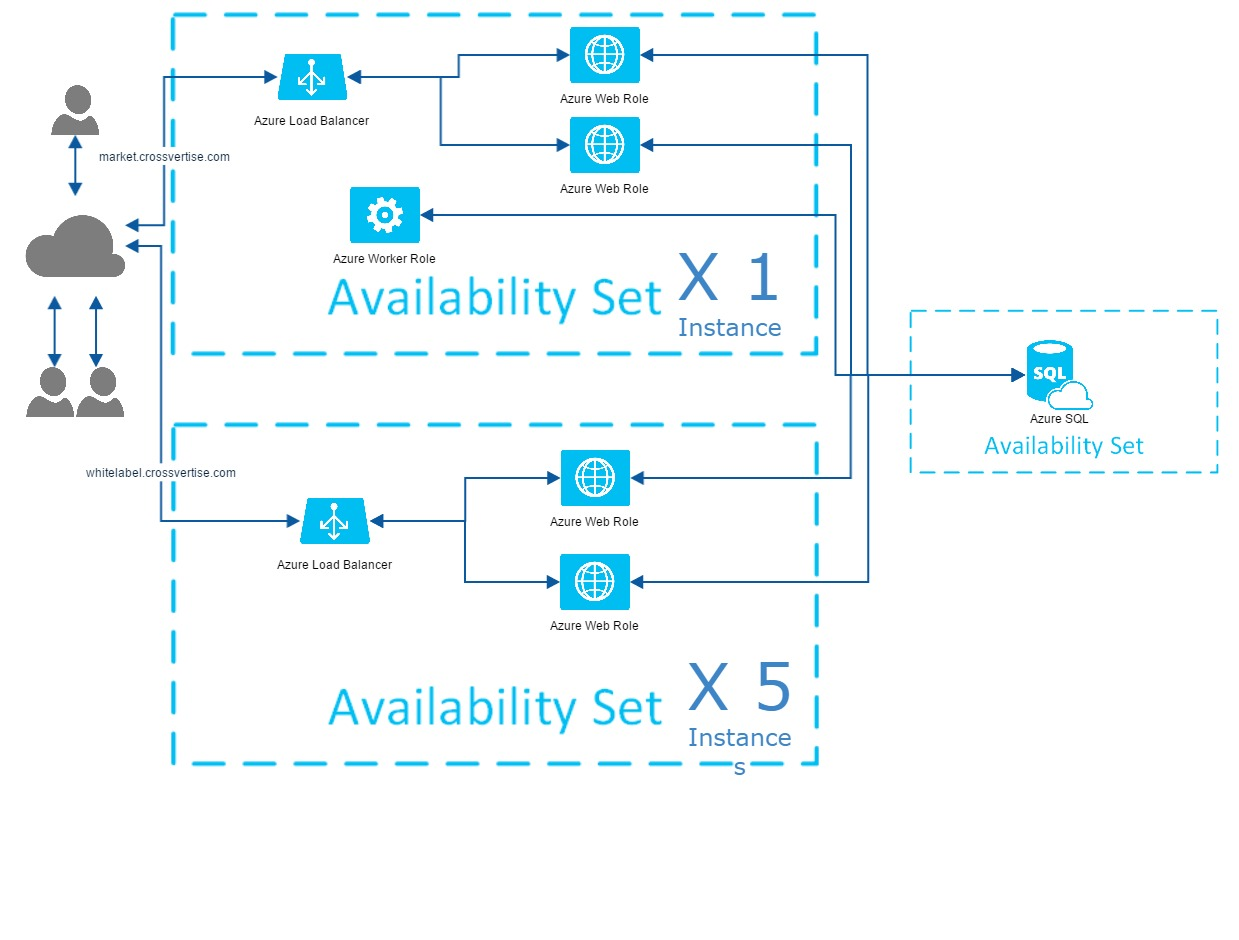
\includegraphics[width=\textwidth]{xv_azure_arc}
\caption{XV Conceptual Architecture Blueprint}
\label{fig:xv_azure_arc}
\end{figure}

\section{The XVA Background}

The current XVA was initially developed as back end to run the companies own media marketplace e-commerce website. However, as time passed it became apparent that they could be a powerful service to be delivered through the public cloud as a SaaS solution for companies that are in the same business domain. Due to this duality in function the application currently only reached SaaS maturity level 1 (ad-hoc) \cite{Chong2006} in the sense that a single, completely customized instance of the application is hosted for each of the application tenants. Since tenants are large advertising companies and have very specific requirements pertaining to the media and mediums which should be provided by their application instance, it has been hard to be able to migrate the service to a higher maturity level. Recently however an active effort has been made by the development team to migrate customization away from code and into configuration in order to achieve SaaS maturity level 2.
 
 
 
At time of writing XV was running 12 instances of their XV Application on Windows Azure Web Roles. Two instances to serve their main website (market.XV.com) and ten instances each serving their individual tenants. Running 12 instances of the same application however is quite costly and has led to the requirement of looking into developing a feasible alternative. The high amount of hosted application instances also contributed to maintenance and administration overhead which could be simplified by a multi-tenant alternative. Finally, the current application persistence model lacks tenant isolation and therefore is a strong candidate for improvement. All of these factors have led to the requirement of moving the current application to a completely scalable, multi-tenant-efficient SaaS solution that meets the criteria of maturity level 4, reduces costs and simplifies tenant provisioning, customization and maintenance.




\subsection{Technical Analysis of the XVA}

As a start-up company, XV has subscribed to Microsoft's BizSpark program which helps start-ups engage in software development by providing them with open access to many of Microsoft's technologies and tools \cite{BizSpark}. This has allowed the company to gain access to the public cloud through Microsoft Azure and develop its application using Visual Studio, C\# and ASP.NET Model, View Controller (MVC). Access to these resources have been the primary decisive factor in choices of technologies used in the application and the current IT team has been structured largely around these Microsoft technologies. It is for these reasons that this research paper has continued to use technologies and tools that align with this strategy, however in cases where newer technologies have become available they have been taken into consideration.
 
 
A more precise breakdown of application technologies can be seen in \ref{fig:tech_breakdown}.

\begin{figure}
\centering
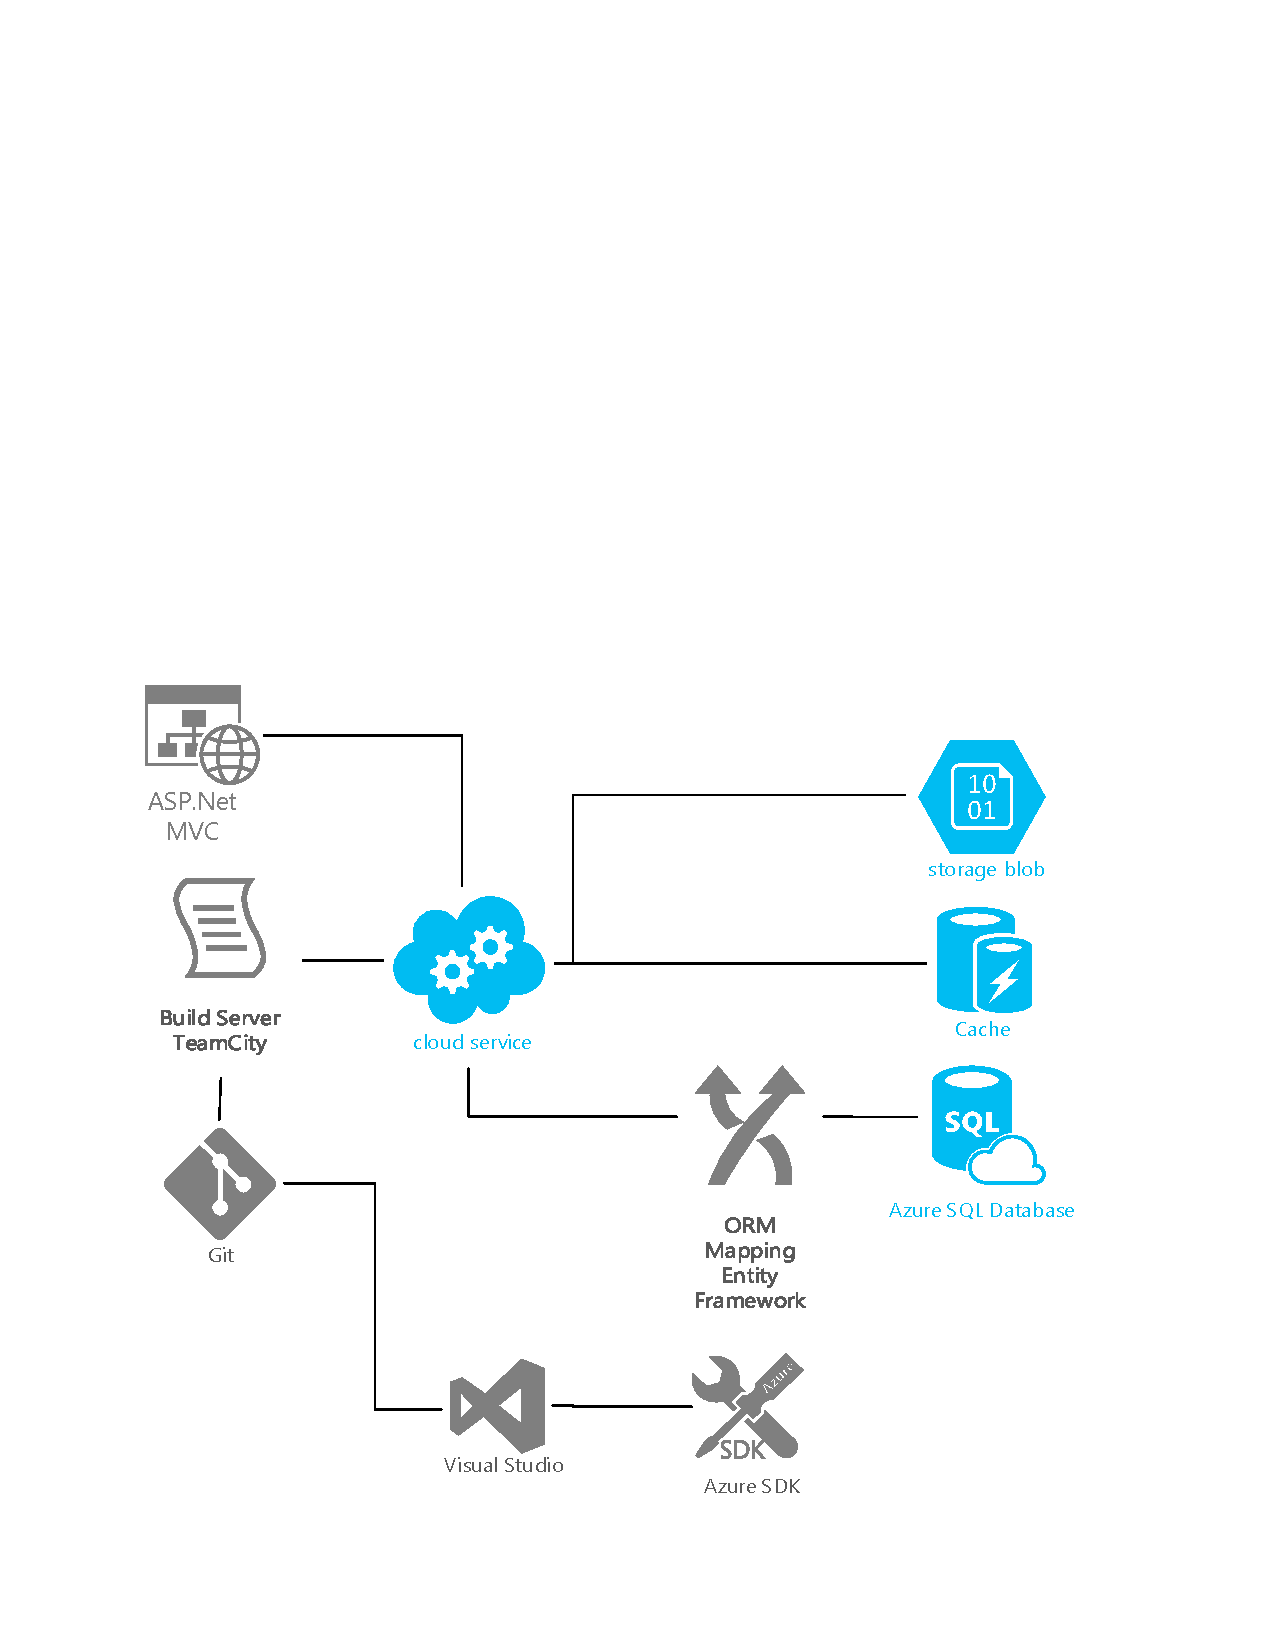
\includegraphics[width=\textwidth]{tech_breakdown}
\caption{XV Technology Breakdown}
\label{fig:tech_breakdown}
\end{figure}

The XVA was designed using the Microsoft's ASP.Net Framework. It utilizes the MVC architectural pattern for the program design and the open source Entity Framework for Object Relational Mapping (ORM) to a collection Microsoft SQL databases. Currently the application is hosted using Microsoft Azure Cloud Services. Website is hosted on Microsoft's Internet Information Services (IIS) installed on an Azure Web Role virtual machine. In conjunction with the Web Role the application uses a helper application running on an Azure Worker Role virtual machine to conduct database, email and other operational tasks. The team uses TeamCity build server for continuous integration and testing and Git and GitHub for source control. Data is persisted to two different Azure SQL Databases, firstly is the marketplace database which stores all of the application e-Commerce transaction and user data and the media database which stores all of the media specific data such as availability, pricing, form factors and publishers. The media DB is quite large (11GB) and is updated every night through the integration of different advertising data outlets and sources. The application stores large binary objects such as videos, images and sounds for the application using Azure Blob storage and uses Azure Cache in order to improve performance. XV currently does not utilize any third party components that would restrict the implementation of a multi-tenant architecture. The majority of code of the XVA was written using C\# (66.3\%) but also includes JavaScript (31.4\%) and Cascading Style Sheets (CSS) (2.1\%) for front-end design.



The application solution consists of 11 projects. The Xv.Marketplace.MVC project includes all MVC code, this includes View Models, Views and Controllers. Although conventional MVC uses models directly within the MVC application, the models for the application have been extracted into the Xv.Marketplace.Domain project. The models are presented using Plain Old CLR Object (POCO) classes combined with Data Annotations that provide the models metadata. The business logic project acts as a service layer and as the name suggest is responsible for all the business logic applied when objects are retrieved from the repositories. The Xv.Marketplace.Worker project is used to complete functional tasks that are not handled by the MVC project such as sending of emails, reminders, cleaning up of storage and indexing. The repositories project is responsible for communicating with the Microsoft SQL database and uses Entity Framework to map objects to a relational database structure and vice versa. The repositories are mostly concerned with Create, Read, Update and Delete (CRUD) operations of entities but also handle security. Finally, the Infrastructure project is used for cross cutting concerns and utilities. This includes resources used in the different projects, helper, wrapper and extension classes. All of the Test projects include either Unit tests for their corresponding projects or in the case of the repositories Test project, integration tests.


\begin{figure}
\centering
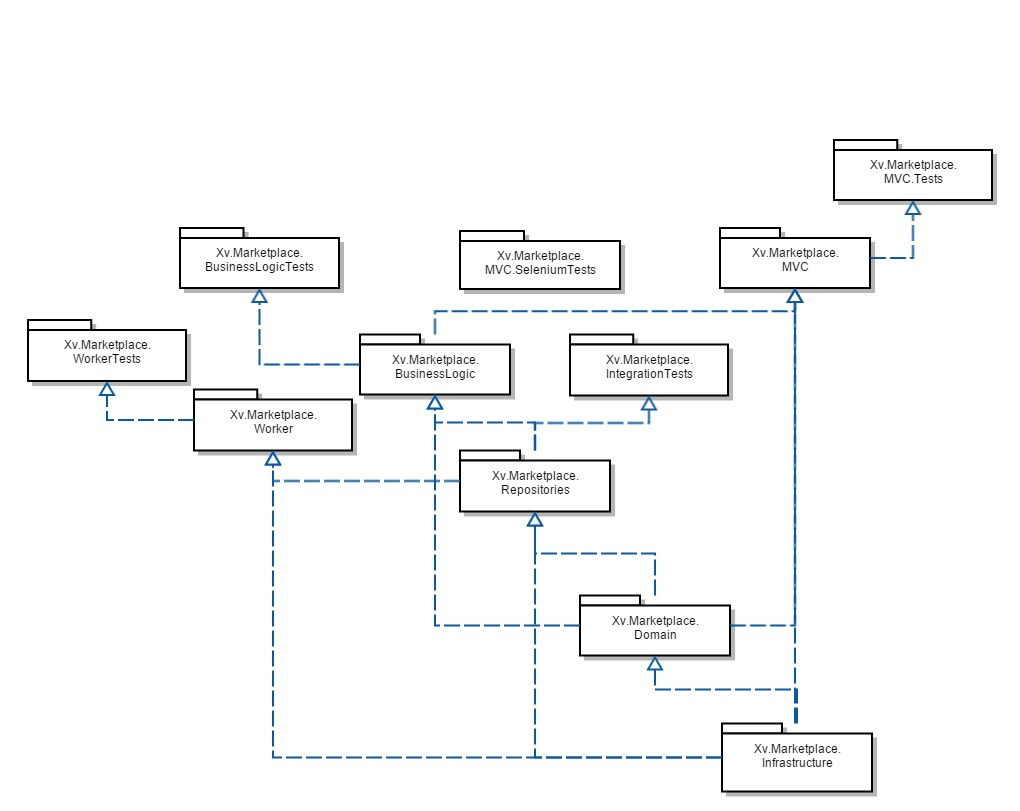
\includegraphics[width=\textwidth]{xv_proj_arc}
\caption{XV Package Diagram}
\label{fig:xv_proj_arc}
\end{figure}


\section{XVA Persistence Schemas}

As the XVA is the Core of the XV business model the exact information regarding the applications database schemas are subject to nondisclosure. In order to provide context for the case study the core tables and relationships in the marketplace database have been extracted and can be seen in Appendix \ref{fig:xv_erd}. The entity relational diagram highlights some important points about the schema used in the current application. Firstly, there is an extreme degree of denormalization used in many of the tables; this has been done in order to improve performance by grouping frequently access data together. Secondly, a lot of multi-directional relationships have developed between the entities as the schema has evolved over time. These relationships are currently a problem as entities can be accessed through multiple roots entities and the current application does not support lazy loading. This causes multiple calls to the database in order to obtain basic child objects. This greatly influences the current persistence performance



\section{Business Requirements}

In addition to the basic technical design requirements, the core business requirement for shifting to a multi-tenant model is reduction of costs. The business model also requires specific provisioning of new tenants/application customers to be streamlined and simplified in order to reduce the amount of developer time required for setting up, customizing and deploying new instances for new tenants. At the current state, provisioning of a new application customer is a long manual process within which the XV Application is manipulated and customized according to the clients' specific needs. This proved to be an extremely time consuming, expensive and resource heavy process. Therefore, one of the fundamental business requirements multi-tenant systems includes high levels of customization with low provisioning costs.



\section{Conclusion}

Throughout this thesis we discuss and articulate means of which to overcome the design requirements defined by this case study. The major requirements including migrating from a SaaS maturity level 1 to a SaaS maturity level 4 implementation. Decreasing overall costs through resource sharing and simplification of the tenant provisioning process. The technological restrictions include using Windows Azure and ASP.NET MVC.